%   Filename    : chapter_4.tex 
\chapter{Preliminary Results/System Prototype}
\section{Overview}
This chapter  presents the preliminary results or the system prototype.  Included in this chapter are screenhots and the discussion of results. The tuna supply chain management smart contract on Hyperledger Fabric has been initiated and tested within a controlled blockchain environment. Results indicated that the system was functionally robust and reliable, having managed assets, transaction integrity, and the ability to query and update the ledger in the blockchain. This chapter presents the details of the major steps executed during the process, results for those steps, and the current status of the prototype's operations. 


\section{Smart Contract Deployment and Installation}

\subsection{Hyperledger Fabric Prerequisites}

Before executing a smart contract framework and blockchain system, it is crucial to first install and set up the necessary tools and technologies. This includes setting up Hyperledger Fabric, which involves installing the Fabric binaries, configuring the network, and ensuring all necessary dependencies like Docker, Docker Compose, and Node.js are installed and properly configured. Additionally, setting up the required certificates, defining the channel configurations, and ensuring that peer nodes and orderers are correctly connected and synchronized are all essential steps in preparing the environment for blockchain and smart contract operations.
\begin{itemize}
	
	\item \textbf{Software Requirements:}
	\begin{itemize}
		\item \textbf{Docker and Docker Compose:} Hyperledger Fabric needs to have Docker installed and running on the system. Docker is required to run the peer and ordering services of the blockchain system.
		\item \textbf{Node.js:} Required for the Fabric SDK for client application integration with JavaScript libraries such as react.
		\item \textbf{Go:} Ensure Go is installed, and the GOPATH environment variable is set up. This is essential for building and running chaincode(smart contract) written in Go.
		\item \textbf{Fabric Samples:} Clone the official Hyperledger Fabric's fabric-samples repository from GitHub:
		\begin{verbatim}
			git clone -b release-2.4 --single-branch 
			https://github.com/hyperledger/fabric-samples
			cd fabric-samples/test-network
		\end{verbatim}
		\item \textbf{Binaries and Docker Images:}
		\begin{verbatim}
			curl -sSL https://bit.ly/2ysbOFE | bash -s
		\end{verbatim}
		
		
	\end{itemize}
	
	
	\item \textbf{Network Setup:}
	\begin{itemize}
		\item Run the \texttt{test-network} script to start the Hyperledger Fabric test network:
		\begin{verbatim}
			./network.sh up
		\end{verbatim}
		This script starts a peer, an ordering service, and a CA (Certificate Authority) on the local machine.
		
		\item After starting the network to docker in the same directory (test-network), a channel must be created:
		\begin{verbatim}
			./network.sh createChannel
		\end{verbatim}
		
	\end{itemize}
	
	\item \textbf{Deploying Chaincode (Smart Contract):}
	\begin{itemize}
		\item Step 1:
		\begin{verbatim}
			export PATH=${PWD}/../bin:$PATH
		\end{verbatim}
		
		\item Step 2:
		\begin{verbatim}
			export FABRIC_CFG_PATH=$PWD/../config/
		\end{verbatim}
		
		\item Step 3:
		\begin{verbatim}
			export CORE_PEER_TLS_ENABLED=true
			export CORE_PEER_LOCALMSPID="Org1MSP"
			export CORE_PEER_TLS_ROOTCERT_FILE=${PWD}/organizations
			/peerOrganizations/org1.example.com/peers/peer0.org1.example.com
			/tls/ca.crt
			export CORE_PEER_MSPCONFIGPATH=${PWD}/organizations
			/peerOrganizations/org1.example.com/users
			/Admin@org1.example.com/msp
			export CORE_PEER_ADDRESS=localhost:7051
			
		\end{verbatim}
		
	\end{itemize}
	
	
\end{itemize}

\subsection{Invoking the Blockchain System}

After setting up the prerequisites, including Docker containers, the test network, and chaincode, the tuna supply chain system can now be invoked for creating, transferring, and querying tuna assets. The figures provided below demonstrate the processes involved in invoking the blockchain system.

	  \begin{figure}[H]
		\centering
		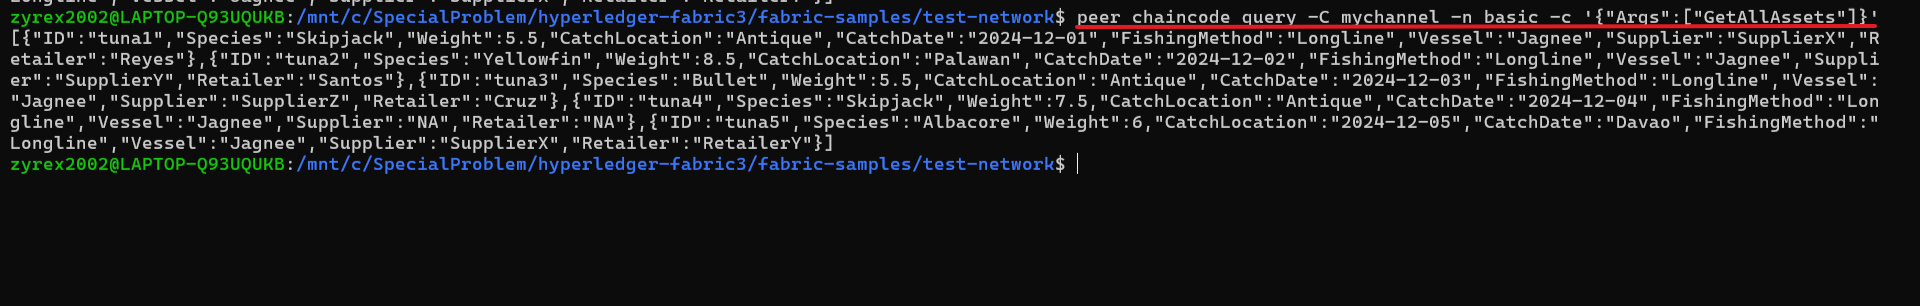
\includegraphics[width=0.8\textwidth]{invoke step 2.png}
		\caption{Query Smart Contract: Check assets}
		\label{fig: second step}
	\end{figure}
	
	\begin{itemize}
	\item \textbf{Adding new tuna assets:}\\
	Here, a new tuna asset is created and registered on the blockchain. This involves invoking the smart contract to add a new entry, which includes details such as the type of tuna, quantity, and any other relevant information. This step ensures that newly caught or acquired tuna can be tracked throughout the supply chain.
	
	\begin{figure}[H]
		\centering
		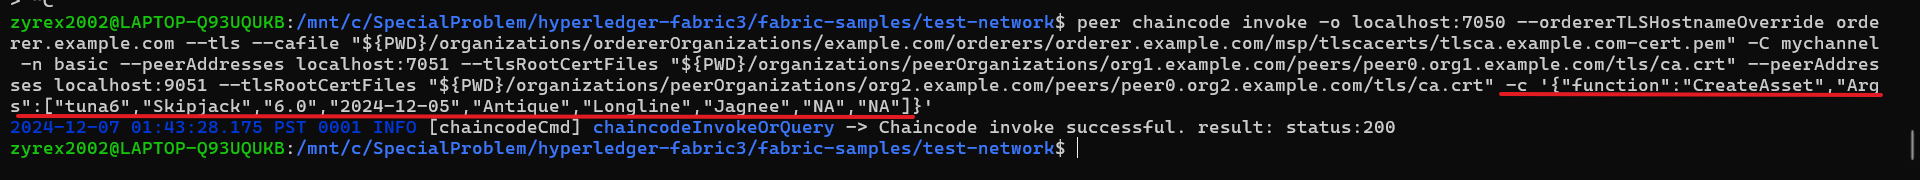
\includegraphics[width=0.8\textwidth]{invoke step 3.png}
		\caption{Invoke Smart Contract: Create/Add new tuna asset}
		\label{fig: third step}
	\end{figure}
	
	\item \textbf{Check all assets after adding a new tuna asset:}\\
	After adding a new tuna asset, the smart contract is queried again to verify that the asset has been successfully added. This step confirms that the new asset is part of the current inventory and that no discrepancies exist in the recorded data.
	
	\begin{figure}[H]
		\centering
		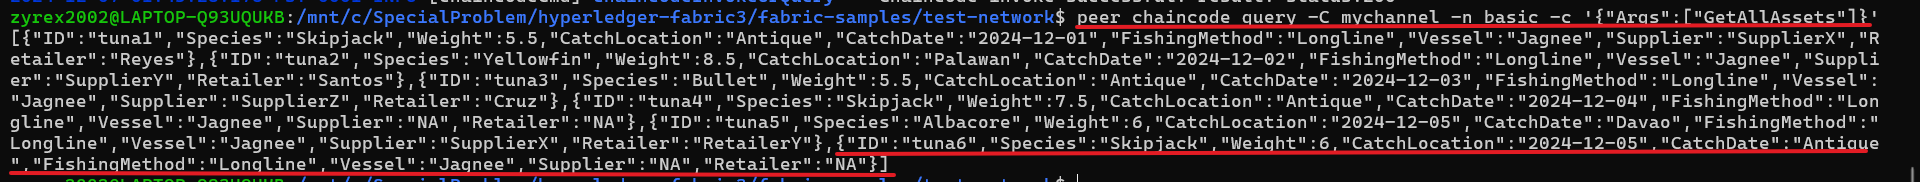
\includegraphics[width=0.8\textwidth]{invoke step 4.png}
		\caption{Query Smart Contract: Check assets with new tuna asset}
		\label{fig: fourth step}
	\end{figure}
	
	\item \textbf{Transfer tuna asset to Supplier:}\\
	This step involves transferring ownership of a tuna asset from the current holder (e.g., a fisherman or a trader) to a supplier. The smart contract is invoked to facilitate the transfer, ensuring that the transaction is securely recorded on the blockchain and that the asset’s new owner is updated accordingly.
	
	\begin{figure}[H]
		\centering
		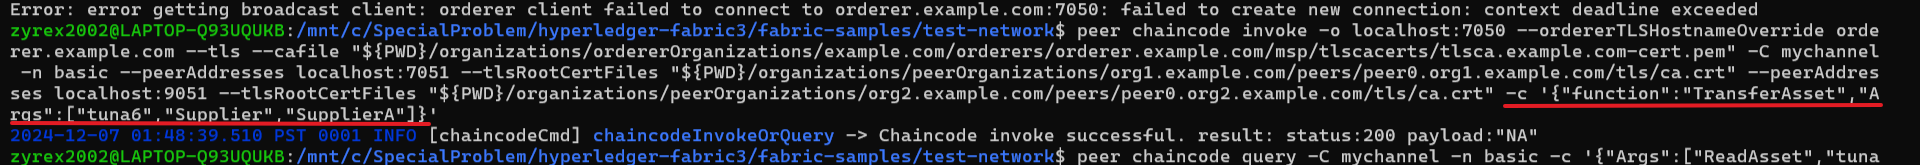
\includegraphics[width=0.8\textwidth]{invoke step 5.png}
		\caption{Invoke Smart Contract: Transfer asset to a supplier}
		\label{fig: fifth step}
	\end{figure}
	
	\item \textbf{Check the updated tuna asset:}\\
	After the transfer, the smart contract is queried once more to check if the asset details have been updated correctly. This step verifies that the asset’s new owner is now the supplier and that all relevant information is correctly updated on the blockchain.
	
	\begin{figure}[H]
		\centering
		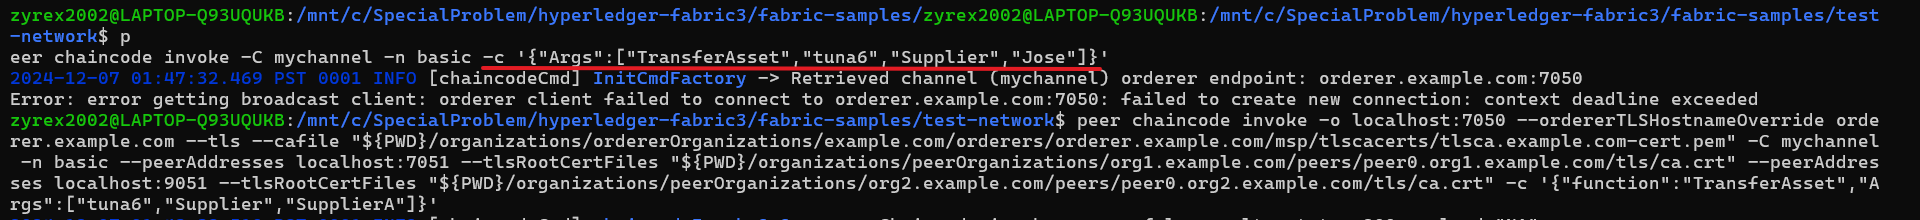
\includegraphics[width=0.8\textwidth]{invoke step 6.png}
		\caption{Query Smart Contract: Check asset after transfer}
		\label{fig: sixth step}
	\end{figure}
	
	\item \textbf{Transfer tuna asset to Retailer:}\\
	Similar to the supplier transfer, this step involves transferring the tuna asset from the supplier to a retailer. The smart contract facilitates this transfer, ensuring that ownership is correctly updated and that the retailer has control over the tuna asset. This step is crucial for the supply chain as it moves the tuna from bulk supply to retail.
	
	\begin{figure}[H]
		\centering
		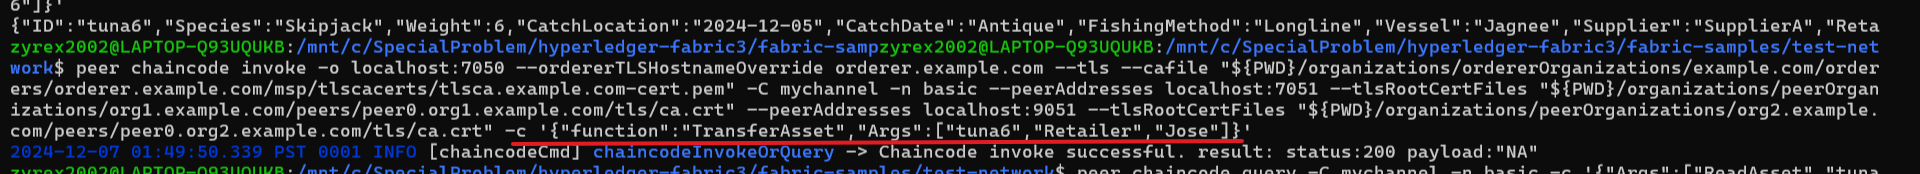
\includegraphics[width=0.8\textwidth]{invoke step 7.png}
		\caption{Invoke Smart Contract: Transfer asset to a retailer}
		\label{fig: seventh step}
	\end{figure}
	
	\item \textbf{Check the updated tuna asset:}\\
	After the transfer to the retailer, another query is made to verify the updated asset details. This step ensures that the transaction was successful and that the retailer now has ownership of the tuna asset. It confirms that the asset has moved through the supply chain correctly.
	
	\begin{figure}[H]
		\centering
		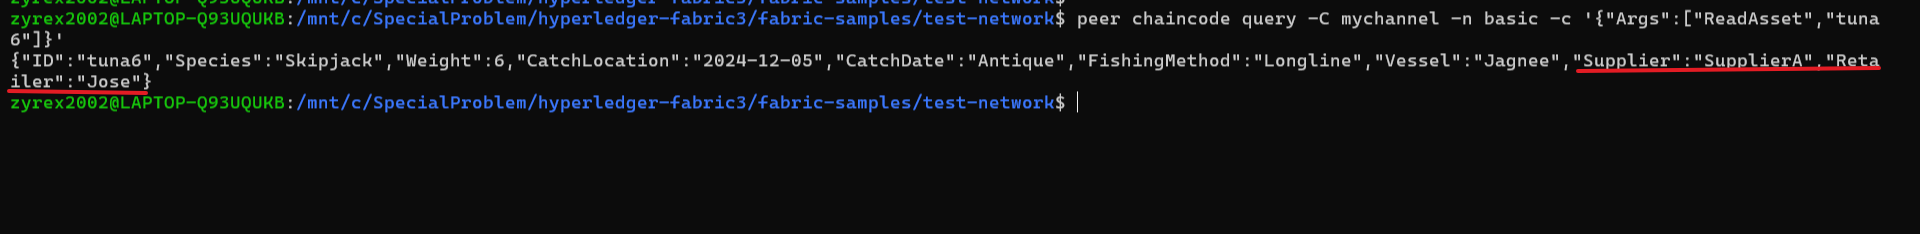
\includegraphics[width=0.8\textwidth]{invoke step 8.png}
		\caption{Query Smart Contract: Check asset after transfer}
		\label{fig: eight step}
	\end{figure}
	
	\item \textbf{Query Smart Contract and check updated assets:}\\
	The final step involves querying the smart contract to get a complete overview of all the assets in the supply chain. This includes all tuna assets from fishing to retail, allowing stakeholders to monitor and manage inventory effectively. It provides transparency in the supply chain, helping to maintain freshness and authenticity of the tuna as it moves through the market.
	
	\begin{figure}[H]
		\centering
		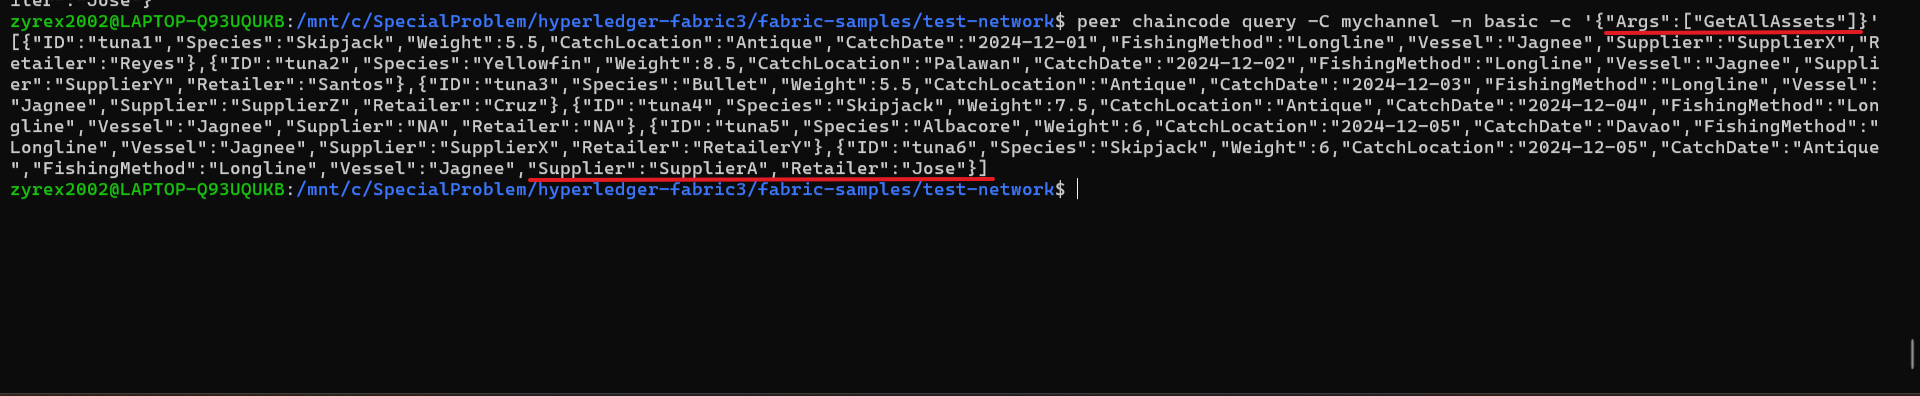
\includegraphics[width=0.8\textwidth]{invoke step 9.png}
		\caption{Query Smart Contract: Check updated assets}
		\label{fig: ninth step}
	\end{figure}
	
		
	\end{itemize}
	
\section{Discussion}
After modifying the Hyperledger Fabric smart contract to assess necessary processes involved in the tuna supply chain, the 
